\documentclass[12pt]{extarticle}
\usepackage{phys440}

\title{PHYS440 - Homework 1+2}
\author{John Hurst}
\date{April 2024}

\hyphenation{trans-pi-la-tion}
\begin{document}
\maketitle

\begin{center}
\noindent\fbox{%
\parbox{0.95\textwidth}{%
Note: As far as I can tell, it is currently not possible to run most circuits created in the IBM Quantum Composer directly on IBM Quantum hardware,
because the Quantum Composer does not support automatic transpilation.
For this reason, I ran all my circuits using Python Qiskit programs, where it is possible to transpile the circuits.
I've included the programs, and images of the original circuits and the transpiled circuits in the submitted files.
}
}
\end{center}

%%%%%%%%%%%%%%%%%%%%%%%%%%%%%%%%%%%%%%%%%%%%%%%%%%%%%%%%%%%%%%%%%%%%%%%%%%%%%%%%%%%%%%%%%%%%%%%%%%%%
\question{1}{Bell-state realization and correlation measurement on \textit{IBM Quantum} (12 marks)

The \textit{Qiskit} textbook chapter on Multiple Qubits and Entangled States explains how to generate the entangled two qubit state
\begin{equation}\label{eq:phiplus}
\ket{\Phi^{+}} = \istwo(\ket{00} + \ket{11})
\end{equation}
and gives the creation of the Bell state
\begin{equation}\label{eq:psiplus}
\ket{\Psi^{+}} = \istwo(\ket{01} + \ket{10})
\end{equation}
as an exercise.
Read this/remind yourself of the relevant material.
Furthermore, read up of how to perform measurements of $Z_0=\idone\otimes Z$ and $Z_1=Z\otimes\idone$
to find the correlator $\langle Z_1Z_0\rangle = P_{00}+P_{11}-P_{01}-P_{10}$.
Use this preparation to answer the following questions.
\begin{enumerate}[(a)]
\item Design the quantum circuits that, starting from the two-qubit state $\ket{00}$, create the remaining two Bell states
\begin{equation}\label{eq:phiminus}
\ket{\Phi^{-}} = \istwo(\ket{00} - \ket{11})
\end{equation}
\begin{equation}\label{eq:psiminus}
\ket{\Psi^{-}} = \istwo(\ket{01} - \ket{10})
\end{equation}
Show (by using matrix representations of the quantum gates) that the circuits that you have designed indeed yield the Bell states as their output.
Submit the circuit diagrams and state-vector simulations from \textit{IBM Quantum} as part of your solution.
\item Consider the two operators $X_0=\idone\otimes X$ and $X_1=X\otimes\idone$.
Design the circuits that allow you to measure
$\langle \Phi^{+}|X_1X_0|\Phi^{+}\rangle$, where $\ket{\Phi^{+}}$ is defined in Eq.~\eqref{eq:phiplus}.
Run the circuit first on the simulator and then on one of the available quantum processors.
Discuss the result of your experiment.
Submit screenshots of your \textit{IBM Quantum} jobs as part of your solution.
\end{enumerate}
}

\begin{enumerate}[(a)]
\item There are a number of different circuits possible for each Bell state.
These two simple examples are perhaps the simplest circuits for $\ket{\Phi^{-}}$ and $\ket{\Psi^{-}}$:

\begin{figure}[H]
\centering
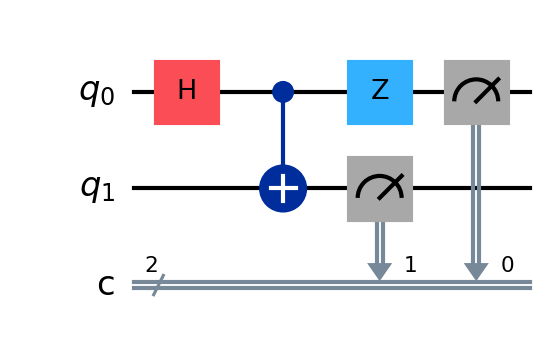
\includegraphics[width=0.80\textwidth]{images/qiskit_phiminus.png}
\caption{Bell state $\ket{\Phi^{-}}$ with Qiskit}
\end{figure}
\begin{figure}[H]
\centering
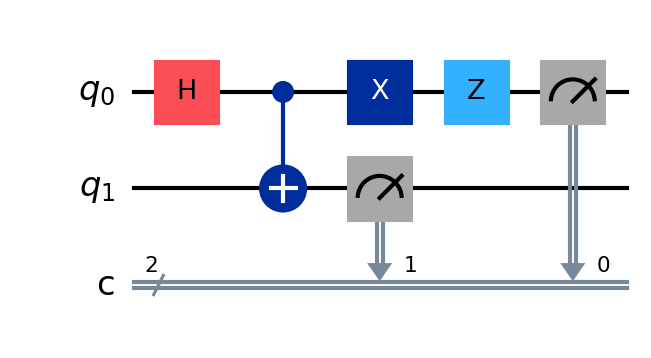
\includegraphics[width=0.80\textwidth]{images/qiskit_psiminus.png}
\caption{Bell state $\ket{\Psi^{-}}$ with Qiskit}
\end{figure}

I ran simple circuits for all four Bell states in the IBM Quantum simulator using the web circuit composer.
The screen shots are included in the submitted files, and the ones for $\ket{\Phi^{-}}$ and $\ket{\Psi^{-}}$ are shown below.

\begin{figure}[H]
\centering
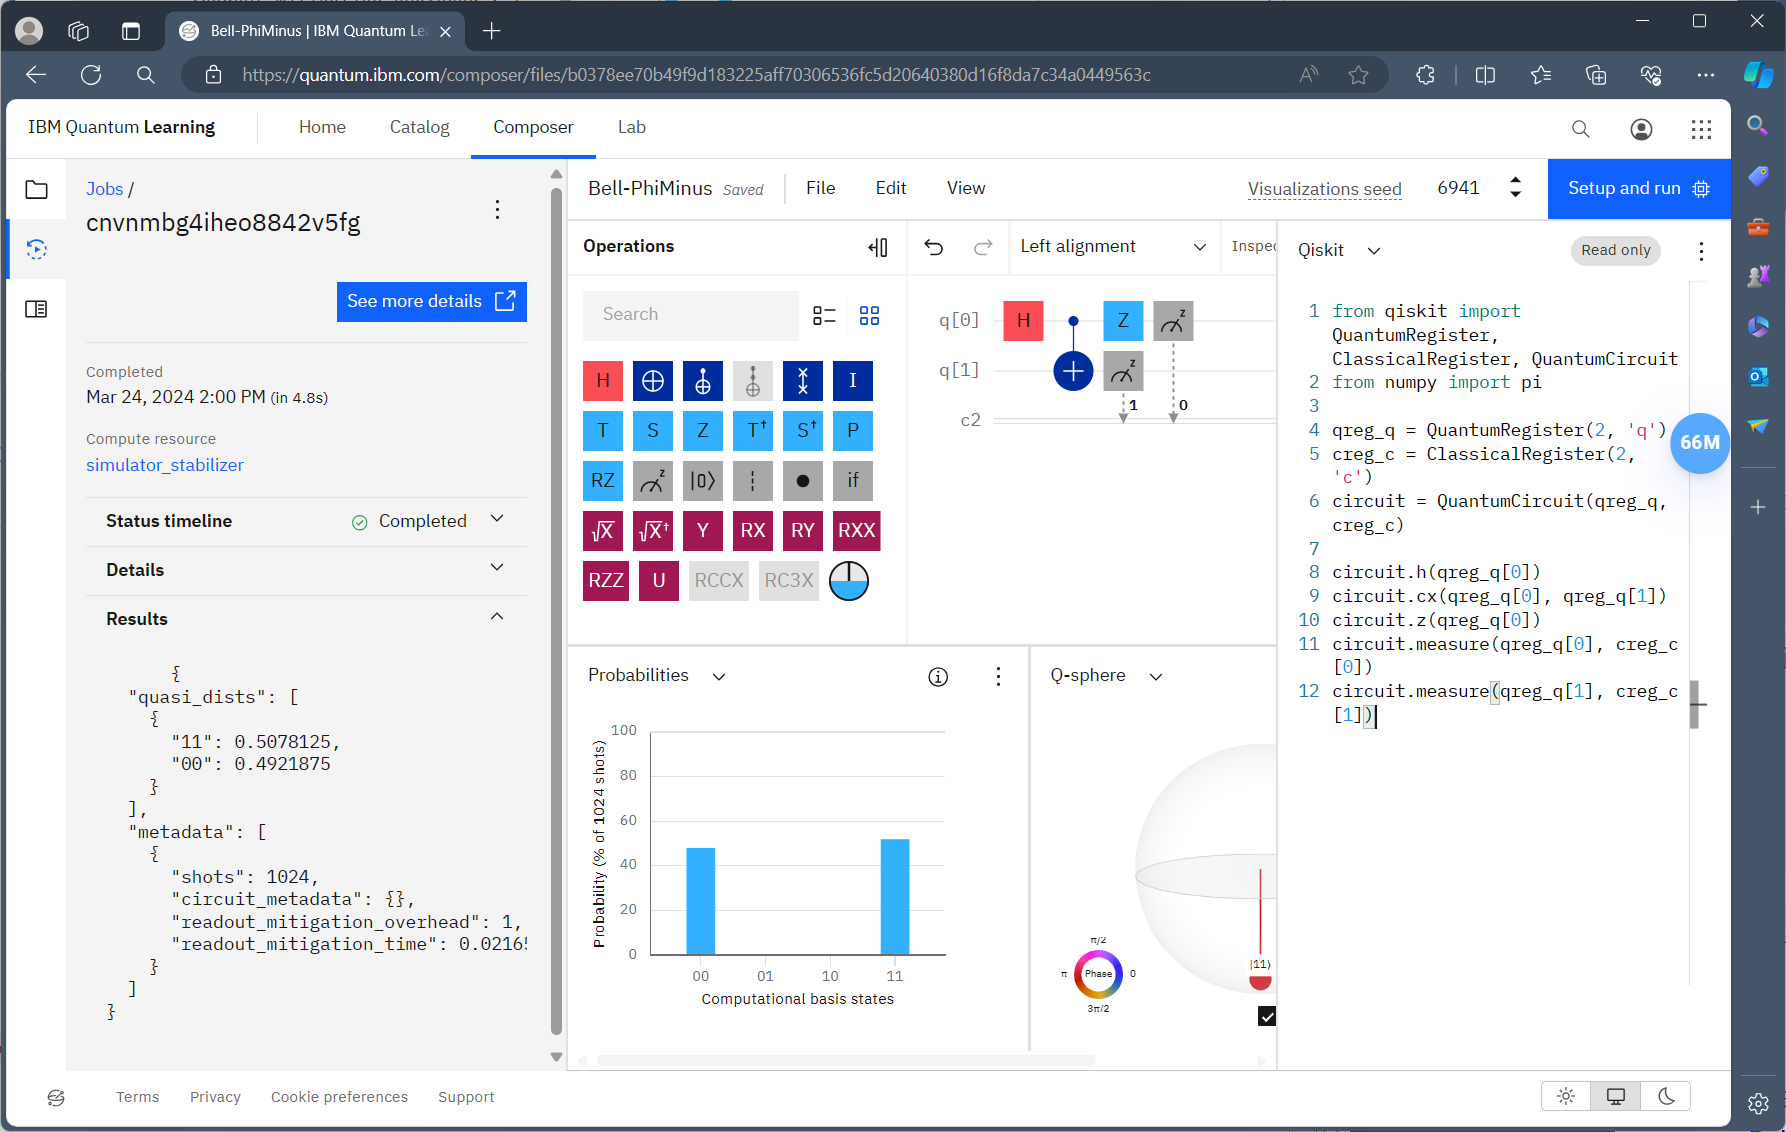
\includegraphics[width=0.80\textwidth]{images/Bell-PhiMinus-IBM-Quantum.png}
\caption{Bell state $\ket{\Phi^{-}}$ on IBM Quantum}
\end{figure}
\begin{figure}[H]
\centering
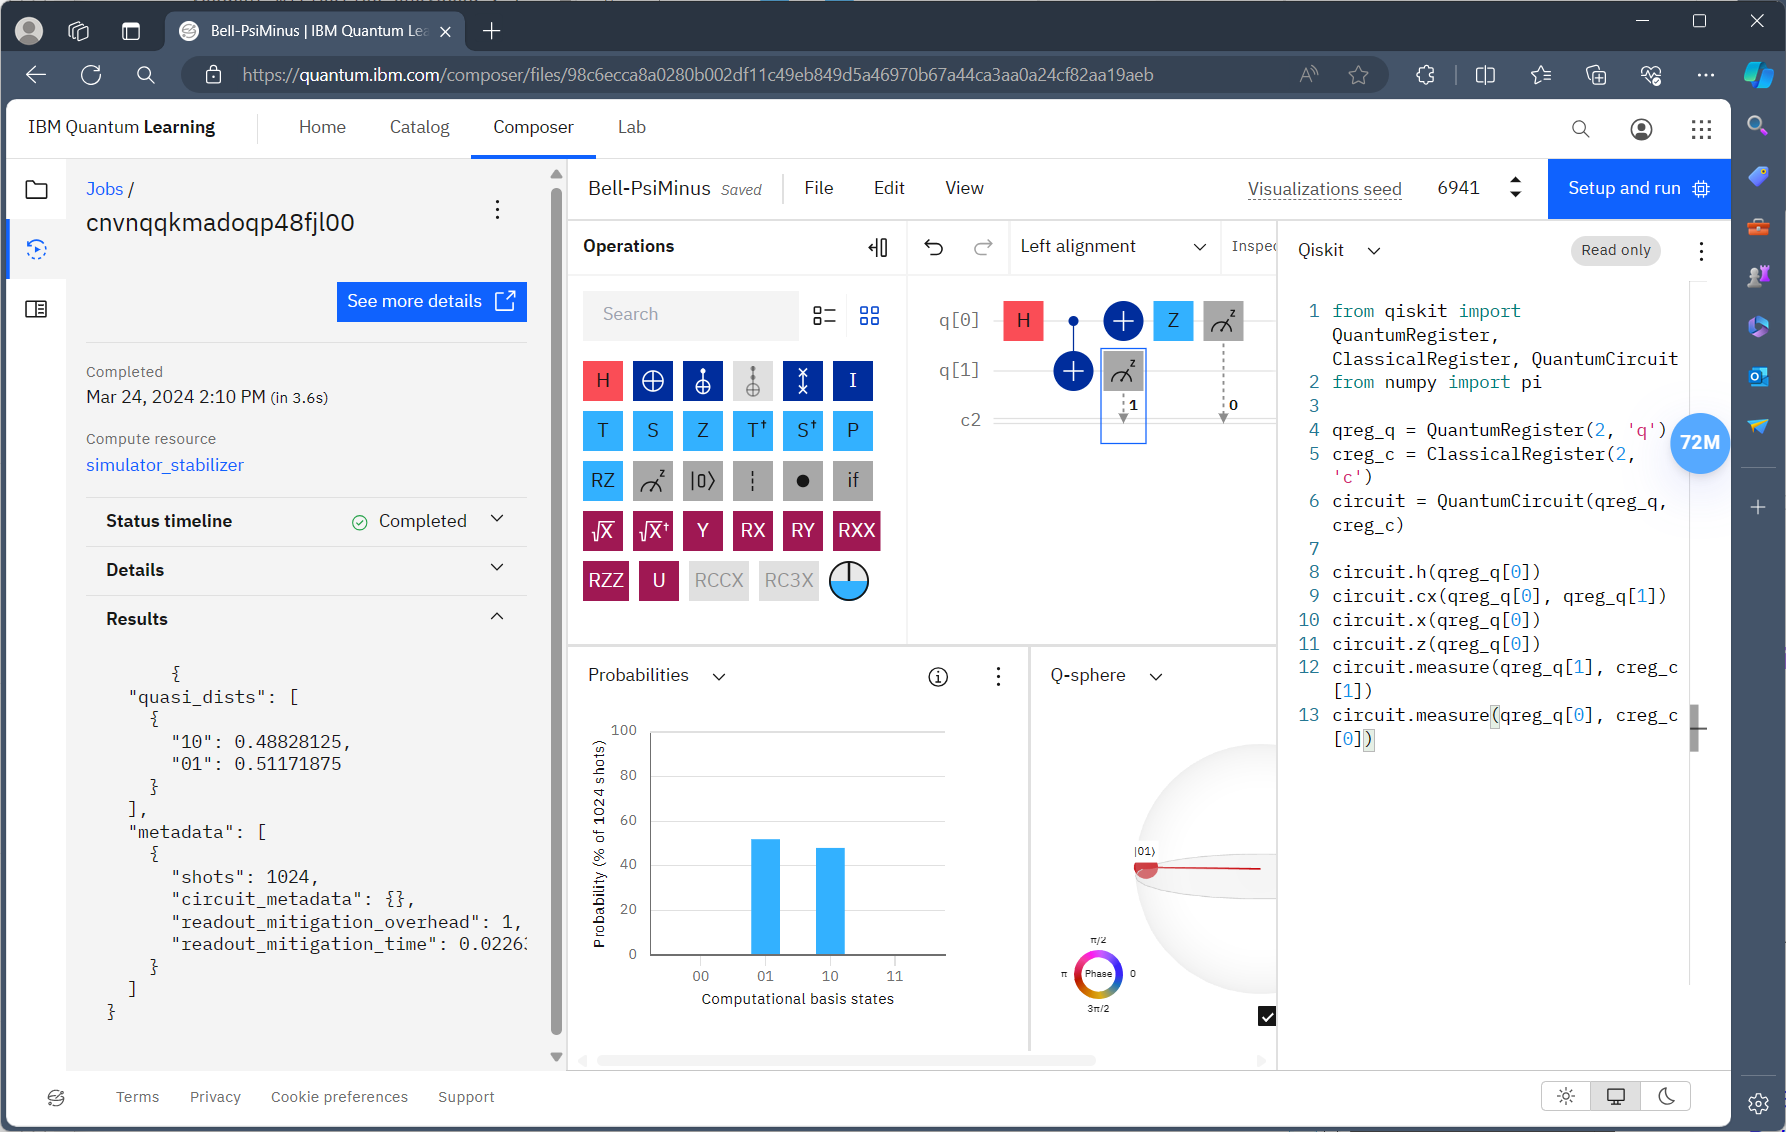
\includegraphics[width=0.80\textwidth]{images/Bell-PsiMinus-IBM-Quantum.png}
\caption{Bell state $\ket{\Psi^{-}}$ on IBM Quantum}
\end{figure}

The IBM Quantum systems follow several architectures, each of which supports only a subset of possible gates.
The Hadamard and CNOT gates are generally not available, and circuits must be designed or transpiled
to use only the available gates.

The attached Mathematica notebook
Homework\_1+2\_Q1a\_BellStates.nb
shows each Bell state created with
simple ``canonical'' circuits (using H and CNOT), and also with circuits using only the gates available on the IBM Quantum systems.
For each circuit the diagram, probability plot, matrix form and output state are shown.

I wrote Python programs using both IBM's Qiskit and Google's Cirq libraries to generate the circuits and simulate them.
The programs are included in the submitted files.

The output of the Qiskit program is:
\begin{lstlisting}[language=bash]
bin/homework12_q1a_qiskit.py --simulate --state=phiplus
00: 0.4893
11: 0.5107
bin/homework12_q1a_qiskit.py --simulate --state=phiminus
00: 0.5195
11: 0.4805
bin/homework12_q1a_qiskit.py --simulate --state=psiplus
01: 0.4717
10: 0.5283
bin/homework12_q1a_qiskit.py --simulate --state=psiminus
01: 0.5029
10: 0.4971
\end{lstlisting}

% Circ program output omitted because of Unicode

% The output of the Circ program is:
% \begin{lstlisting}[language=bash]
% bin/homework12_q1a_cirq.py --phiplus
% 0: ───H───@───
%           │
% 1: ───────X───
% measurements: (no measurements)

% qubits: (cirq.LineQubit(0), cirq.LineQubit(1))
% output vector: 0.707|00⟩ + 0.707|11⟩

% phase:
% output vector: |⟩

% bin/homework12_q1a_cirq.py --phiminus
% 0: ───H───@───Z───
%           │
% 1: ───────X───────
% measurements: (no measurements)

% qubits: (cirq.LineQubit(0), cirq.LineQubit(1))
% output vector: 0.707|00⟩ - 0.707|11⟩

% phase:
% output vector: |⟩

% bin/homework12_q1a_cirq.py --psiplus
% 0: ───H───@───X───
%           │
% 1: ───────X───────
% measurements: (no measurements)

% qubits: (cirq.LineQubit(0), cirq.LineQubit(1))
% output vector: 0.707|01⟩ + 0.707|10⟩

% phase:
% output vector: |⟩

% bin/homework12_q1a_cirq.py --psiminus
% 0: ───H───@───X───Z───
%           │
% 1: ───────X───────────
% measurements: (no measurements)

% qubits: (cirq.LineQubit(0), cirq.LineQubit(1))
% output vector: 0.707|01⟩ - 0.707|10⟩

% phase:
% output vector: |⟩
% \end{lstlisting}

The Qiskit version of the program also supports running on the real IBM Quantum hardware, using the Qiskit \texttt{Sampler} feature.
This includes a transpilation step to convert the circuit to use only the available gates.
I captured the transpiled circuits and the results of running them on the IBM Quantum hardware.
Because the transpiled circuits include a very large number of ancilla bits, I have cropped the images to show only the relevant parts.
I've included the images in the submitted files.

Once the jobs are completed, I queried the results:
\begin{lstlisting}[language=bash]
bin/qiskit_job_status.py cr48fcd0dz600086ntg0
Status: JobStatus.DONE
Backend: ibm_osaka
Tags: ['homework12', 'bell', 'phiplus', 'ibm_osaka']
Sample data for pub 0: {'11': 498, '00': 492, '01': 13, '10': 21}

bin/qiskit_job_status.py cr499xz8091g008jnn80
Status: JobStatus.DONE
Backend: ibm_osaka
Tags: ['homework12', 'bell', 'phiminus', 'ibm_osaka']
Sample data for pub 0: {'11': 469, '01': 35, '00': 491, '10': 29}

bin/qiskit_job_status.py cr49ba52yk500082p5f0
Status: JobStatus.DONE
Backend: ibm_osaka
Tags: ['homework12', 'bell', 'psiplus', 'ibm_osaka']
Sample data for pub 0: {'10': 424, '00': 84, '01': 447, '11': 69}

bin/qiskit_job_status.py cr49c6g0dz600086nwk0
Status: JobStatus.DONE
Backend: ibm_osaka
Tags: ['homework12', 'bell', 'psiminus', 'ibm_osaka']
Sample data for pub 0: {'10': 391, '01': 398, '00': 147, '11': 88}
\end{lstlisting}

The results are summarised in the table below, as proportions:
\begin{center}
\begin{tabular}{|c|c|c|c|c|}
\hline
Bell state & $\ket{00}$ & $\ket{01}$ & $\ket{10}$ & $\ket{11}$ \\
\hline
$\ket{\Phi^{+}}$ & 48\% &  1\% &  2\% & 49\% \\
$\ket{\Phi^{-}}$ & 48\% &  3\% &  3\% & 46\% \\
$\ket{\Psi^{+}}$ &  8\% & 44\% & 41\% &  7\% \\
$\ket{\Psi^{-}}$ & 14\% & 39\% & 38\% &  9\% \\
\hline
\end{tabular}
\end{center}

The results illustrate the presence of noise, because there are a significant number of counts for the states that should not be present.


% And also these circuit images:
% \begin{figure}[H]
% \centering
% 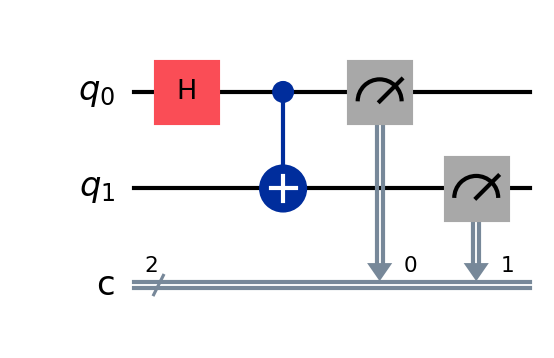
\includegraphics[width=0.50\textwidth]{images/qiskit_phiplus.png}
% \caption{Bell state $\ket{\Phi^{+}}$ on local simulator}
% \end{figure}
% \begin{figure}[H]
% \centering
% 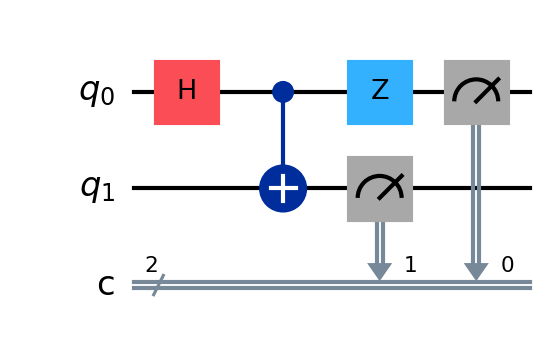
\includegraphics[width=0.50\textwidth]{images/qiskit_phiminus.png}
% \caption{Bell state $\ket{\Phi^{-}}$ on local simulator}
% \end{figure}
% \begin{figure}[H]
% \centering
% 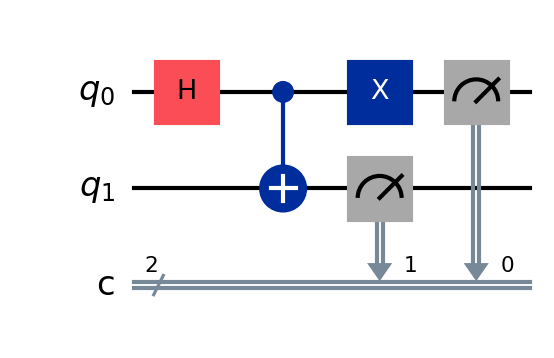
\includegraphics[width=0.50\textwidth]{images/qiskit_psiplus.png}
% \caption{Bell state $\ket{\Psi^{+}}$ on local simulator}
% \end{figure}
% \begin{figure}[H]
% \centering
% 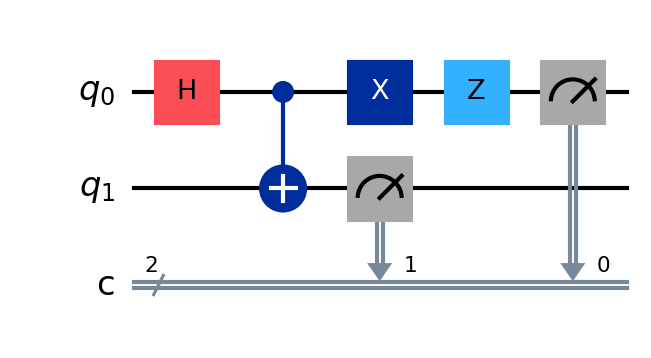
\includegraphics[width=0.50\textwidth]{images/qiskit_psiminus.png}
% \caption{Bell state $\ket{\Psi^{-}}$ on local simulator}
% \end{figure}

\item We can compute $X_0$ and $X_1$ and the correlator as:
\begin{align*}
X_0 & = \idone\otimes X = \begin{pmatrix}1&0\\0&1\end{pmatrix}\otimes\begin{pmatrix}0&1\\1&0\end{pmatrix} = \begin{pmatrix}0&1&0&0\\1&0&0&0\\0&0&0&1\\0&0&1&0\end{pmatrix} \\
X_1 & = X\otimes\idone = \begin{pmatrix}0&1\\1&0\end{pmatrix}\otimes\begin{pmatrix}1&0\\0&1\end{pmatrix} = \begin{pmatrix}0&0&1&0\\0&0&0&1\\1&0&0&0\\0&1&0&0\end{pmatrix} \\
X_1X_0 & = \begin{pmatrix}0&0&1&0\\0&0&0&1\\1&0&0&0\\0&1&0&0\end{pmatrix}\begin{pmatrix}0&1&0&0\\1&0&0&0\\0&0&0&1\\0&0&1&0\end{pmatrix} \\
& = \begin{pmatrix}0&0&0&1\\0&0&1&0\\0&1&0&0\\1&0&0&0\end{pmatrix}
\end{align*}

We can compute $\langle \Phi^{+}|X_1X_0|\Phi^{+}\rangle$ as:
\begin{align*}
\langle \Phi^{+}|X_1X_0|\Phi^{+}\rangle
& = \frac{1}{\sqrt{2}}\begin{pmatrix}1&0&0&1\end{pmatrix}
\begin{pmatrix}0&0&0&1\\0&0&1&0\\0&1&0&0\\1&0&0&0\end{pmatrix}
\frac{1}{\sqrt{2}} \begin{pmatrix}1\\0\\0\\1\end{pmatrix} \\
& = \frac{1}{2}\begin{pmatrix}1&0&0&1\end{pmatrix} \begin{pmatrix}1\\0\\0\\1\end{pmatrix} \\
& = \frac{1}{2}(1+1) \\
& = 1
\end{align*}

The included Mathematica notebook Homework\_1+2\_Q1b\_CorrelationExpectation.nb verifies this analytic calculation.

It also includes a simple quantum circuit to measure the correlator $\langle \Phi^{+}|X_1X_0|\Phi^{+}\rangle$.

I also wrote a Python program using Qiskit Sampler feature to generate the circuit and simulate it.

The circuit run by the program is shown below:

\begin{figure}[H]
\centering
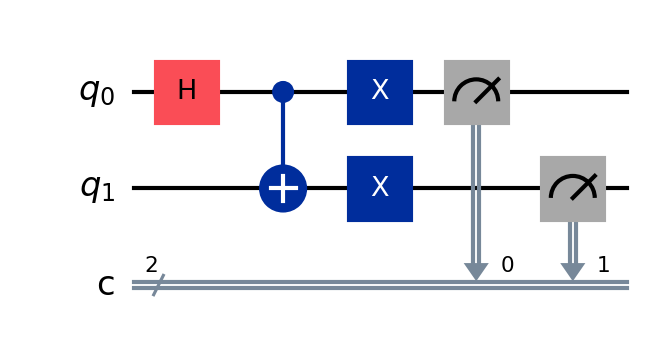
\includegraphics[width=0.80\textwidth]{images/xcorrelator_qiskit.png}
\caption{Bell state $\ket{\Phi^{-}}$ with Qiskit}
\end{figure}

Running the program in simulation mode:

\begin{lstlisting}[language=bash]
bin/homework12_q1b_qiskit.py --simulate --filename=xcorrelator_qiskit.png
00: 0.4746
11: 0.5254
\end{lstlisting}

This shows a clean result with perfect expectation of 1, as expected.

I also ran the program on the IBM Quantum hardware, and the results are shown below:

\begin{lstlisting}[language=bash]
bin/homework12_q1b_qiskit.py --run --pass-manager --filename=xcorrelator_qiskit_ibmquantum_full.png
# ... wait for job to complete
bin/qiskit_job_status.py cr6z43r95ey00083jtf0
Status: JobStatus.DONE
Backend: ibm_brisbane
Tags: ['homework12', 'xcorrelator', 'ibm_brisbane']
Sample data for pub 0: {'11': 504, '00': 454, '01': 45, '10': 21}
\end{lstlisting}

The results are summarised in the table below, as proportions:

\begin{center}
\begin{tabular}{|c|c|c|c|c|}
\hline
State vector & $\ket{00}$ & $\ket{01}$ & $\ket{10}$ & $\ket{11}$ \\
\hline
Frequency & 44\% &  4\% &  2\% & 49\% \\
\hline
\end{tabular}
\end{center}

These results also show the presence of noise, with a significant number of counts for the states that should not be present.

We can also do this experiment more simply in Qiskit using the Estimator feature instead of the Sampler feature.

With the Estimator, we only need to do the circuit to prepare the input state, $\ket{\Phi^{+}}$:
\begin{lstlisting}[language=python]
circuit = QuantumCircuit(2)
circuit.h(0)
circuit.cx(0, 1)
\end{lstlisting}
Then we can define the observable and run the experiment:
\begin{lstlisting}[language=python]
# Define observable as 1 * X_1 * X_0.
observable = SparsePauliOp.from_list([("XX", 1)])
\end{lstlisting}

My program can run this in the simulator:
\begin{lstlisting}[language=bash]
bin/homework12_q1b_qiskit_estimator.py --simulate
[1.]
\end{lstlisting}

This again gives a perfect result of 1.0.

I also ran the program on the IBM Quantum hardware, and the results are shown below:
\begin{lstlisting}[language=bash]
bin/homework12_q1b_qiskit_estimator.py --run \
  --filename=xcorrelator_qiskit_estimator_ibmquantum_full.png
# ... wait for job to complete
bin/qiskit_job_status.py crct7hpdjmqg008kemeg
Status: JobStatus.DONE
Backend: ibm_osaka
Tags: None
Estimate data for pub 0: [[1.0078125]]
\end{lstlisting}

The result is 1.0078125, which is very close to the expected value of 1.0, but shows the presence of noise.

\end{enumerate}

%%%%%%%%%%%%%%%%%%%%%%%%%%%%%%%%%%%%%%%%%%%%%%%%%%%%%%%%%%%%%%%%%%%%%%%%%%%%%%%%%%%%%%%%%%%%%%%%%%%%
\question{2}{Testing Bell's Inequality on \textit{IBM Quantum} (28 marks)

To answer the questions below, it will be useful to first familiarise yourself with the CHSH inequality,
e.g. by reading about it in textbooks and/or the document \textit{A Brief Introduction to Entanglement \& the CHSH inequality} from our \texttt{Lit} folder.
You will also have to make use of the techniques learned from Question 1 above.

Consider the state $\ket{\Psi^{-}} = \istwo(\ket{01}-\ket{10})$ and the following observables
\begin{align*}
A & = Z\otimes \idone \quad ; & A' & = X\otimes \idone \\
B & = \idone \otimes \istwo(X+Z) \quad ; & B' & = \idone \otimes \istwo(X-Z).
\end{align*}

\begin{enumerate}[(a)]
\item Calculate analytically, using the matrix representation of the relevant quantum gates, the following correlators:
\begin{equation}\label{eq:correlators}
\langle \Psi^{-}|AB|\Psi^{-}\rangle, \quad \langle \Psi^{-}|AB' |\Psi^{-}\rangle , \quad \langle \Psi^{-}|A'B|\Psi^{-}\rangle, \quad \langle \Psi^{-}|A'B'|\Psi^{-}\rangle,
\end{equation}
as well as the quantity
\begin{equation}\label{eq:c}
C = \langle \Psi^{-}|AB|\Psi^{-}\rangle - \langle \Psi^{-}|AB' |\Psi^{-}\rangle + \langle \Psi^{-}|A'B|\Psi^{-}\rangle + \langle \Psi^{-}|A'B'|\Psi^{-}\rangle.
\end{equation}
\item Design the four quantum circuits that will allow you to measure the expectation values given in Eq.~\eqref{eq:correlators}.
Submit the circuit diagrams from \textit{IBM Quantum} as part of your solution.
\item Run the circuits on the simulator, evaluate the expectation values from Eq.~\eqref{eq:correlators},
and check whether the CHSH inequality is violated.
Submit screenshots of your \textit{IBM Quantum} jobs as part of your solution.
\item Now run your circuits on one of the available quantum processors and evaluate the expectation values from Eq.~\eqref{eq:correlators} as well as $|C|$,
with $C$ given in Eq.~\eqref{eq:c}.
\item Submit screenshots of your \textit{IBM Quantum} jobs as part of your solution.
\item Comment on your result, discussing specifically whether---and if so, at what level of confidence---it rules out the possibility of a hidden variable theory.
\end{enumerate}
}

\begin{enumerate}[(a)]
\item
The included Mathematica notebook Homework\_1+2\_Q2\_CHSH.nb calculates the correlators and the CHSH quantity $C$ analytically.

It gives a result of $C = -2\sqrt{2}$, or $|C| = 2\sqrt{2}$, which violates the CHSH inequality.
This is actually the maximum violation predicted by quantum mechanics, according to the Tsirelson bound.

\item
I used the four circuits shown below.
Each circuit prepares the input state of $\ket{\Psi^{-}}$ and then performs the necessary transformation of the quantum state into the computational (Z) basis to perform the measurement of the desired observable.

\begin{itemize}
\item To measure $A=Z_0$ requires no transformation, because $Z_0$ is already in the computational basis.
\item To measure $A'=X_0$ requires a Hadamard gate on qubit 0 before the measurement.
\item To measure $B=\frac{1}{\sqrt{2}}(X_1 + Z_1)$ requires a $Y$ rotation of $-\frac{\pi}{4}$, achieved by the RY($-\frac{\pi}{4}$) gate.
\item I was not completely sure about the transformation required to measure $B'=\frac{1}{\sqrt{2}}(X_1 - Z_1)$, but it appears that
RY($-\frac{\pi}{4}$) followed by a Hadamard gate is the correct transformation.
\end{itemize}

\begin{figure}[H]
\centering
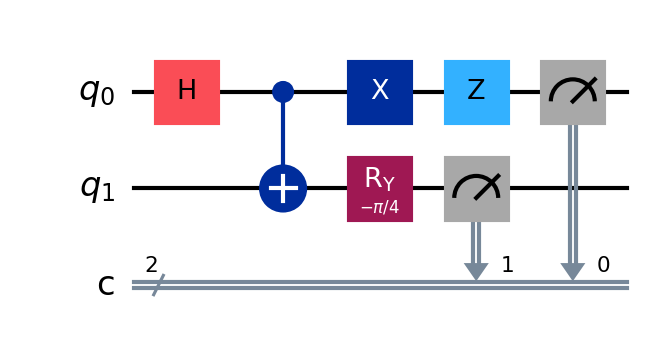
\includegraphics[width=0.80\textwidth]{images/chsh_ab_qiskit.png}
\caption{Circuit for measuring $\langle \Psi^{-}|AB|\Psi^{-}\rangle$}
\end{figure}
\begin{figure}[H]
\centering
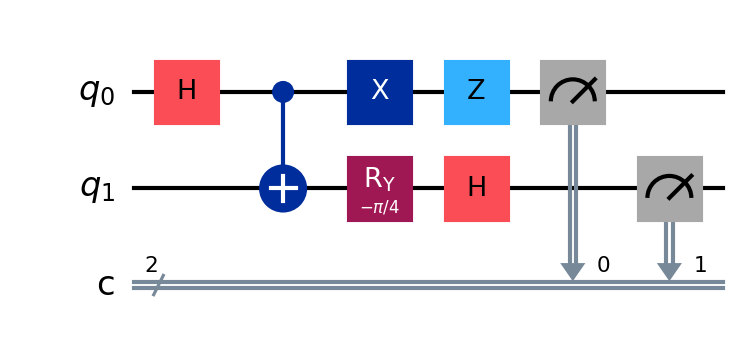
\includegraphics[width=0.80\textwidth]{images/chsh_abp_qiskit.png}
\caption{Circuit for measuring $\langle \Psi^{-}|AB'|\Psi^{-}\rangle$}
\end{figure}
\begin{figure}[H]
\centering
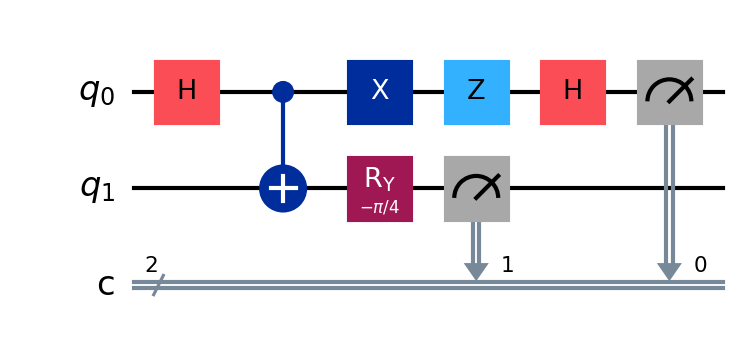
\includegraphics[width=0.80\textwidth]{images/chsh_apb_qiskit.png}
\caption{Circuit for measuring $\langle \Psi^{-}|A'B|\Psi^{-}\rangle$}
\end{figure}
\begin{figure}[H]
\centering
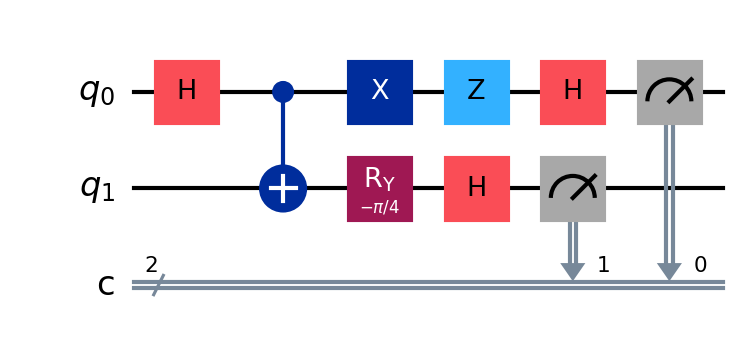
\includegraphics[width=0.80\textwidth]{images/chsh_apbp_qiskit.png}
\caption{Circuit for measuring $\langle \Psi^{-}|A'B'|\Psi^{-}\rangle$}
\end{figure}

The Mathematica notebook referenced above also evaluates the expectations for the observables using these circuits,
and shows that the circuits give the same result as the analytic calculation.

\item

I wrote a Python program using the Qiskit Sampler feature to generate the circuits and simulate them.

The program runs the circuits and prints the statevector frequency proportions:

\begin{lstlisting}[language=bash]
bin/homework12_q2_qiskit.py --obs=ab --simulate
00: 0.0811
01: 0.4160
10: 0.4336
11: 0.0693
bin/homework12_q2_qiskit.py --obs=abp --simulate
00: 0.4326
01: 0.0684
10: 0.0742
11: 0.4248
bin/homework12_q2_qiskit.py --obs=apb --simulate
00: 0.0723
01: 0.4336
10: 0.4219
11: 0.0723
bin/homework12_q2_qiskit.py --obs=apbp --simulate
00: 0.0654
01: 0.4287
10: 0.4355
11: 0.0703
\end{lstlisting}

We use these proportions to calculate the expectation values for the observables using
\[
\langle AB \rangle = P_{00} - P_{01} - P_{10} + P_{11}
\]
as shown in this table:

\begin{center}
\begin{tabular}{|c|r|r|r|r|r|}
\hline
Observable & $P_{00}$ & $P_{01}$ & $P_{10}$ & $P_{11}$ & $P_{00} - P_{01} - P_{10} + P_{11}$ \\
\hline
AB   & 0.0811 & 0.4160 & 0.4336 & 0.0693 & -0.6992 \\
AB'  & 0.4326 & 0.0684 & 0.0742 & 0.4248 &  0.7148 \\
A'B  & 0.0723 & 0.4336 & 0.4219 & 0.0723 & -0.7109 \\
A'B' & 0.0654 & 0.4287 & 0.4355 & 0.0703 & -0.7285 \\
\hline
\end{tabular}
\end{center}

The CHSH quantity $C$ is then calculated as:
\begin{align*}
C & = \langle AB \rangle - \langle AB' \rangle + \langle A'B \rangle + \langle A'B' \rangle \\
& = -0.6992 - 0.7148 - 0.7109 - 0.7285 \\
& = -2.8534
\end{align*}

This result is close to the analytic result of $-2\sqrt{2} \approx -2.8284$.

% I studied Nielsen and Chuang\cite{nielsen2016} ``EPR and the Bell inequality'', which has an example very similar to this problem.
% I also looked at the IBM tutorial\cite{ibm_chsh}, which uses a parameterized circuit that generalises this question and checks the inequality over a range of parameters.

% The books by Wong\cite{wong2022} and Silva\cite{silva2024} both contain extensive examples of a different variation of the CHSH inequality, using slightly more complex observables.
% Although they show the circuits and the computation of the expectation values in detail, I could not see how to relate the expectations back to the analytic versions.

% However, I was able to make some progress using the Estimator feature in Qiskit.
% (I found it by following the IBM tutorial.)

The Qiskit Estimator feature is a simpler way to compute the expectations required in this question,
because it requires only the definition of a single circuit (for the input state only),
and the Estimator takes care of the rest.

I wrote a separate Python program to use the Estimator feature to compute the expectations.
The program is included in the submitted files, but the important parts are shown below.

We prepare the entangled qubits in the state $\ket{\Psi^{-}}$:
\begin{lstlisting}[language=python]
chsh_circuit = QuantumCircuit(2)
chsh_circuit.h(0)
chsh_circuit.cx(0, 1)
chsh_circuit.x(0)
chsh_circuit.z(0)
\end{lstlisting}

Then we define the observables that we are interested in:
\begin{align*}
AB & = Z_0 \times \frac{1}{\sqrt{2}} (X_1 + Z_1) = \frac{1}{\sqrt{2}} (X_1 Z_0 + Z_1 Z_0) \\
AB' & = Z_0 \times \frac{1}{\sqrt{2}} (X_1 - Z_1) = \frac{1}{\sqrt{2}} (X_1 Z_0 - Z_1 Z_0) \\
A'B & = X_0 \times \frac{1}{\sqrt{2}} (X_1 + Z_1) = \frac{1}{\sqrt{2}} (X_1 X_0 + Z_1 X_0) \\
A'B' & = X_0 \times \frac{1}{\sqrt{2}} (X_1 - Z_1) = \frac{1}{\sqrt{2}} (X_1 X_0 - Z_1 X_0) \\
C & = AB - AB' + A'B + A'B' \\
& = \frac{1}{\sqrt{2}}(X_1 Z_0 + Z_1 Z_0) - \frac{1}{\sqrt{2}} (X_1 Z_0 - Z_1 Z_0) \\
& \qquad + \frac{1}{\sqrt{2}} (X_1 X_0 + Z_1 X_0) + \frac{1}{\sqrt{2}} (X_1 X_0 - Z_1 X_0) \\
& = \sqrt{2} Z_1 Z_0 + \sqrt{2} X_1 X_0 \\
\end{align*}
Technically it would be sufficient to define only $C$, but I've included the others as required by the question and to show more detail.
\begin{small}
\begin{lstlisting}[language=python]
observable_ab =
    SparsePauliOp.from_list([("XZ", 1/sqrt(2)), ("ZZ", 1/sqrt(2))])
observable_abp =
    SparsePauliOp.from_list([("XZ", 1/sqrt(2)), ("ZZ", -1/sqrt(2))])
observable_apb =
    SparsePauliOp.from_list([("XX", 1/sqrt(2)), ("ZX", 1/sqrt(2))])
observable_apbp =
    SparsePauliOp.from_list([("XX", 1/sqrt(2)), ("ZX", -1/sqrt(2))])
observable_c =
    SparsePauliOp.from_list([("ZZ", sqrt(2)), ("XX", sqrt(2))])
\end{lstlisting}
\end{small}

We run the circuit using the Qiskit simulator, and evaluate the expectation values:

\begin{lstlisting}[language=bash]
bin/homework12_q2_qiskit_estimator.py --simulate
[-0.70710678  0.70710678 -0.70710678 -0.70710678 -2.82842712]
\end{lstlisting}

These results agree perfectly with the analytic results:

\begin{align*}
\langle \Psi^{-}|AB|\Psi^{-}\rangle & = -\frac{1}{\sqrt{2}} \\
\langle \Psi^{-}|AB'|\Psi^{-}\rangle & = \frac{1}{\sqrt{2}} \\
\langle \Psi^{-}|A'B|\Psi^{-}\rangle & = -\frac{1}{\sqrt{2}} \\
\langle \Psi^{-}|A'B'|\Psi^{-}\rangle & = -\frac{1}{\sqrt{2}} \\
C & = -2\sqrt{2}
\end{align*}

\item

I ran the individual circuits using the Sampler feature on IBM Quantum hardware.
The transpiled circuit diagrams are included in the submitted files.

The first run generated these counts:

\begin{center}
\begin{tabular}{|c|c|r|r|r|r|}
\hline
Observable & Backend & $\ket{00}$ & $\ket{01}$ & $\ket{10}$ & $\ket{11}$  \\
\hline
AB   & ibm\_kyoto & 178 & 306 & 304 & 236 \\
AB'  & ibm\_kyoto & 307 & 170 & 158 & 389 \\
A'B  & ibm\_osaka & 115 & 412 & 413 &  84 \\
A'B' & ibm\_osaka & 119 & 414 & 403 &  88 \\
\hline
\end{tabular}
\end{center}

We convert these counts to proportions and calculate the expectation values:

\begin{center}
\begin{tabular}{|c|r|r|r|r|r|}
\hline
Observable & $P_{00}$ & $P_{01}$ & $P_{10}$ & $P_{11}$ & $P_{00} - P_{01} - P_{10} + P_{11}$ \\
\hline
AB   & 0.1738 & 0.2988 & 0.2969 & 0.2305 & -0.1914 \\
AB'  & 0.2998 & 0.1660 & 0.1543 & 0.3799 &  0.3594 \\
A'B  & 0.1123 & 0.4023 & 0.4033 & 0.0820 & -0.6113 \\
A'B' & 0.1162 & 0.4043 & 0.3936 & 0.0859 & -0.5957 \\
\hline
\end{tabular}
\end{center}

The CHSH quantity $C$ is then calculated as:
\begin{align*}
C & = \langle AB \rangle - \langle AB' \rangle + \langle A'B \rangle + \langle A'B' \rangle \\
& = -0.1914 - 0.3594 - 0.6113 - 0.5957 \\
& = -1.7578
\end{align*}

So, from this experiment we get $|C|<2$, which does not violate the CHSH inequality.
However, this result might have been affected by noise in the IBM Quantum systems.
I ran the same circuits a second time, and happened to get them run on a different combination of IBM Quantum backends:

\begin{center}
\begin{tabular}{|c|c|r|r|r|r|}
\hline
Observable & Backend & $\ket{00}$ & $\ket{01}$ & $\ket{10}$ & $\ket{11}$  \\
\hline
AB   & ibm\_osaka & 118 & 399 & 427 &  80 \\
AB'  & ibm\_osaka & 434 &  98 &  98 & 394 \\
A'B  & ibm\_osaka &  98 & 425 & 423 &  78 \\
A'B' & ibm\_kyoto & 151 & 343 & 345 & 185 \\
\hline
\end{tabular}
\end{center}

This time the proportions were more consistent with the analytic and simulator results:

\begin{center}
\begin{tabular}{|c|r|r|r|r|r|}
\hline
Observable & $P_{00}$ & $P_{01}$ & $P_{10}$ & $P_{11}$ & $P_{00} - P_{01} - P_{10} + P_{11}$ \\
\hline
AB   & 0.1152 & 0.3896 & 0.4170 & 0.0781 & -0.6133 \\
AB'  & 0.4238 & 0.0957 & 0.0957 & 0.3848 &  0.6172 \\
A'B  & 0.0957 & 0.4150 & 0.4131 & 0.0762 & -0.6563 \\
A'B' & 0.1475 & 0.3350 & 0.3369 & 0.1807 & -0.3438 \\
\hline
\end{tabular}
\end{center}

Now, the CHSH quantity $C$ is calculated as:
\begin{align*}
C & = -0.6133 - 0.6172 - 0.6563 - 0.3438 \\
& = -2.2306
\end{align*}

This result does violate the CHSH inequality, but it is still less than the maximum violation predicted by quantum mechanics.

It appears that the ibm\_koyoto backend did not give very good results for these circuits at the time I ran them,
while the ibm\_osaka backend gave more consistent results.

I also ran the Estimator version of the program on the IBM Quantum hardware:

\begin{small}
\begin{lstlisting}[language=bash]
bin/homework12_q2_qiskit_estimator.py --run \
    --filename=chsh_qiskit_estimator_ibmquantum_full.png
# ... wait for job to complete
bin/qiskit_job_status.py crcwnppdqdn000834ksg
Status: JobStatus.DONE
Backend: ibm_osaka
Tags: ['homework12', 'chsh', 'ibm_osaka']
Estimate data for pub 0: [[-0.65312916  0.77907694 -0.73409559
  -0.7376941  -2.90399579]]
\end{lstlisting}
\end{small}

The numbers are similar to the simulator results, but again show the presence of noise in the IBM Quantum system.

\item

Interestingly, the result from the IBM Quantum system using the Estimator has $|C|=2.90$, which is actually greater than
the $2\sqrt{2}\approx 2.83$ maximum violation predicted by quantum mechanics.

According to theory, a result greater than 2 implies that the system is not compatible with a local hidden variable theory.
However, given the obvious noise issues, I am not sure what level of confidence we can assign to this result.
Although the deviation is large (larger even than quantum mechanics predicted!), our experiments on IBM Quantum
have displayed a large amount of unexpected results due to noise.
I'm not sure we can apply any formal statistical analysis to this result, without accounting for the statistical properties of the noise.

\end{enumerate}

% \printbibliography
% \addcontentsline{toc}{section}{References}

\end{document}
